\documentclass[11pt]{article}

% ----- preamble (matches the other notes in this project) -----
\usepackage[a4paper,margin=1.9cm]{geometry}
\usepackage{amsmath,amssymb}
\usepackage{array}
\usepackage{booktabs}
\usepackage{tikz}
\usepackage{tikz-cd}
\usetikzlibrary{arrows.meta,positioning,calc,fit,backgrounds,
  shapes.geometric,chains,decorations.pathreplacing}
\usepackage[most]{tcolorbox}
\usepackage{parskip}
\usepackage{xcolor}

\definecolor{ink}{RGB}{40,40,40}
\definecolor{soft}{RGB}{245,245,248}
\definecolor{kas}{RGB}{30,110,190}
\definecolor{grn}{RGB}{30,140,80}

% the three brick colours used across this project's picture books
\definecolor{faceL}{RGB}{30,140,80}   % linearized trace  L
\definecolor{faceF}{RGB}{200,140,0}   % Frobenius / doubling  F
\definecolor{faceC}{RGB}{130,70,170}  % cyclotomic coset bookkeeping  C

\newtcolorbox{note}[1][]{colback=soft,colframe=ink,boxrule=0.4pt,
  arc=2pt,left=6pt,right=6pt,top=4pt,bottom=4pt,#1}
\newtcolorbox{leanbox}[1][]{colback=black!4,colframe=black!55,boxrule=0.4pt,
  arc=1.5pt,left=5pt,right=5pt,top=3pt,bottom=3pt,#1}

\tikzset{
  vtx/.style={circle,draw=ink,fill=soft,minimum size=6.5mm,font=\small,inner sep=0pt},
  fld/.style={circle,draw=faceF,fill=faceF!12,minimum size=6.5mm,font=\small,inner sep=0pt},
  arr/.style={-{Stealth[length=2.4mm]},thick},
  uarr/.style={thick},
  badge/.style={circle,inner sep=0pt,minimum size=3.8mm,font=\scriptsize\bfseries,text=white},
}
\newcommand{\bL}{\tikz[baseline=-0.6ex]\node[badge,fill=faceL]{L};}
\newcommand{\bF}{\tikz[baseline=-0.6ex]\node[badge,fill=faceF]{F};}
\newcommand{\bC}{\tikz[baseline=-0.6ex]\node[badge,fill=faceC]{C};}

\newcommand{\tr}{\operatorname{tr}}
\newcommand{\Tr}{\operatorname{Tr}}
\newcommand{\id}{\mathrm{id}}
\newcommand{\lc}[1]{\texttt{\small #1}}
\newcommand{\smallmat}[1]{\left(\begin{smallmatrix}#1\end{smallmatrix}\right)}

\title{\vspace{-1.4cm}\textbf{Traces, Powers, and Closed Patterns}\\[3pt]
\large Adjacency matrices as relations --- and how the same loop reappears
in the Frobenius trace of this project\\[2pt]
\normalsize \bL~linearized trace \quad \bF~Frobenius \quad \bC~cyclotomic cosets}
\author{\small A follow-up picture book, in plain English, with categories and TikZ}
\date{}

\begin{document}
\maketitle
\vspace{-0.9cm}

\begin{note}
\textbf{One idea, three costumes.} The trace of a matrix adds up its diagonal;
that already \emph{counts self-relations} ($x\,R\,x$). Raise the matrix to a
power first and the diagonal counts something richer --- \textbf{closed walks},
i.e.\ patterns that return to where they started. Categorically this is nothing
but \emph{feedback}: the trace of $R^{k}$ picks out the points fixed by
composing the relation $k$ times. The punchline for \emph{this} formalisation:
the Frobenius map $x\mapsto x^{2}$ is itself an endorelation, its ``feedback''
cycles are exactly the cyclotomic cosets~\bC, and the project's trace
$\Tr(x)=\sum_{i<n}x^{2^{i}}$~\bL\ is the very same categorical loop applied to
``multiply by $x$''.
\end{note}

\hrule
\section*{1. The trace already counts self-relations}

Let $R$ be a relation on a finite set $\{1,\dots,n\}$: write $a_{ij}=1$ when
$i\,R\,j$ and $0$ otherwise. The array $A=(a_{ij})$ is the
\textbf{adjacency matrix}, and a relation is literally the same data as its
$0/1$ matrix. Its trace is
\[
\tr(A)=\sum_{i} a_{ii}=\#\{\,i : i\,R\,i\,\}=\text{number of self-loops.}
\]
So before any powers appear, the trace is already a counting statement:

\begin{center}
\begin{tabular}{@{}l@{\qquad}l@{}}
\emph{Reflexive} ($x\,R\,x$ always) & $\tr(A)=n$ \\[2pt]
\emph{Irreflexive} (never $x\,R\,x$) & $\tr(A)=0$
\end{tabular}
\end{center}

\begin{center}
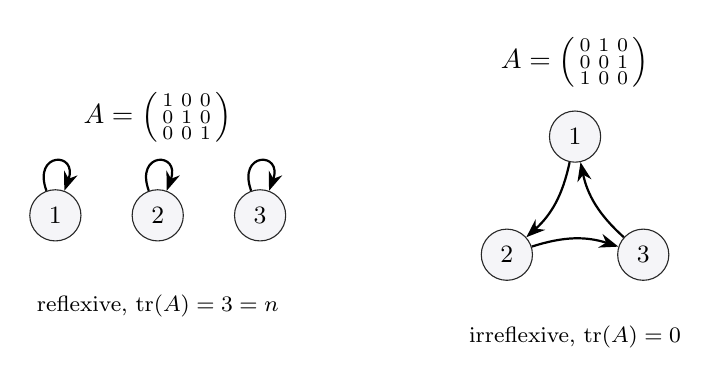
\begin{tikzpicture}[node distance=13mm]
% Reflexive: 3 nodes, each a self loop
\begin{scope}
  \node[vtx] (a1) at (0,0) {1};
  \node[vtx] (a2) at (1.3,0) {2};
  \node[vtx] (a3) at (2.6,0) {3};
  \foreach \n in {a1,a2,a3}{\draw[arr] (\n) to[out=110,in=70,looseness=6] (\n);}
  \node at (1.3,-1.15) {\footnotesize reflexive, $\tr(A)=3=n$};
  \node at (1.3,1.25) {$A=\smallmat{1&0&0\\0&1&0\\0&0&1}$};
\end{scope}
% Irreflexive: directed 3-cycle
\begin{scope}[xshift=6.6cm]
  \node[vtx] (b1) at (90:1) {1};
  \node[vtx] (b2) at (210:1) {2};
  \node[vtx] (b3) at (330:1) {3};
  \draw[arr] (b1) to[bend left=18] (b2);
  \draw[arr] (b2) to[bend left=18] (b3);
  \draw[arr] (b3) to[bend left=18] (b1);
  \node at (0,-1.55) {\footnotesize irreflexive, $\tr(A)=0$};
  \node at (0,1.95) {$A=\smallmat{0&1&0\\0&0&1\\1&0&0}$};
\end{scope}
\end{tikzpicture}
\end{center}

\section*{2. Powers of the matrix compose the relation}

Multiplying adjacency matrices \emph{composes} relations. The Boolean reading
is ``there is a step'': $(A^{2})_{ij}\neq0$ exactly when some $k$ has
$i\,R\,k\,R\,j$. The linear-algebra reading \emph{counts the ways}:
\[
(A^{k})_{ij}=\#\{\text{walks } i\to\cdots\to j \text{ of length }k\}.
\]
Putting $j=i$ and summing the diagonal gives the headline formula.

\begin{note}
\[
\boxed{\;\tr(A^{k})=\sum_{i}(A^{k})_{ii}
=\#\{\text{closed walks of length }k\}.\;}
\]
Each closed walk starts and ends at the same vertex; equivalently it is a
\textbf{fixed point of $R^{k}=R\circ\cdots\circ R$}, i.e.\ a cycle whose length
divides $k$.
\end{note}

\paragraph{$k=2$ detects symmetry.}
Since $(A^{2})_{ii}=\sum_j a_{ij}a_{ji}$, each term is $1$ precisely when
$i\leftrightarrow j$ is a \emph{mutual} pair. So $\tr(A^{2})$ measures how
symmetric the relation is; for an undirected graph every edge is counted twice,
$\tr(A^{2})=2\cdot(\#\text{edges})=\sum_i \deg(i)$.

\paragraph{$k=3$ counts triangles.}
$\tr(A^{3})$ counts closed walks of length $3$; for an undirected simple graph
each triangle is walked $6$ ways (3 starts $\times$ 2 directions), so
$\#\text{triangles}=\tr(A^{3})/6$.

\begin{center}
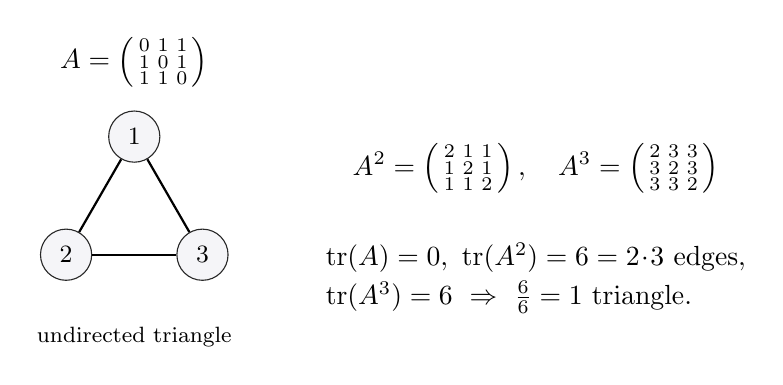
\begin{tikzpicture}
% undirected triangle
\begin{scope}
  \node[vtx] (c1) at (90:1)  {1};
  \node[vtx] (c2) at (210:1) {2};
  \node[vtx] (c3) at (330:1) {3};
  \draw[uarr] (c1)--(c2); \draw[uarr] (c2)--(c3); \draw[uarr] (c3)--(c1);
  \node at (0,-1.55) {\footnotesize undirected triangle};
  \node at (0,1.95) {$A=\smallmat{0&1&1\\1&0&1\\1&1&0}$};
\end{scope}
% computed traces
\begin{scope}[xshift=5.1cm,yshift=-0.1cm]
  \node[align=left] at (0,0.7)
    {$A^{2}=\smallmat{2&1&1\\1&2&1\\1&1&2},\quad
      A^{3}=\smallmat{2&3&3\\3&2&3\\3&3&2}$};
  \node[align=left] at (0,-0.7)
    {$\tr(A)=0,\ \tr(A^{2})=6=2\!\cdot\!3\text{ edges},$\\[2pt]
     $\tr(A^{3})=6\ \Rightarrow\ \tfrac{6}{6}=1\text{ triangle.}$};
\end{scope}
\end{tikzpicture}
\end{center}

\noindent For the \emph{directed} $3$-cycle of \S1, instead $\tr(A)=\tr(A^{2})=0$
but $A^{3}=I$, so $\tr(A^{3})=3$: three vertices each return after three
directed steps --- one directed triangle, walked from each of its $3$ starts.

\section*{3. A dictionary: relation properties $\leftrightarrow$ traces}

\begin{center}
\renewcommand{\arraystretch}{1.35}
\begin{tabular}{@{}l l l@{}}
\toprule
\textbf{Property} & \textbf{Matrix condition} & \textbf{Trace role}\\
\midrule
Reflexive & $a_{ii}=1$ & $\tr(A)=n$\\
Irreflexive & $a_{ii}=0$ & $\tr(A)=0$\\
Symmetric & $A=A^{\mathsf T}$ & large $\tr(A^{2})$ (every mutual pair counts)\\
Antisymmetric & $a_{ij}a_{ji}=0\ (i\neq j)$ & $\tr(A^{2})=\tr(A)$\\
Transitive & $A^{2}\le A$ (Boolean product) & \emph{no} simple trace formula\\
\bottomrule
\end{tabular}
\end{center}

\begin{center}
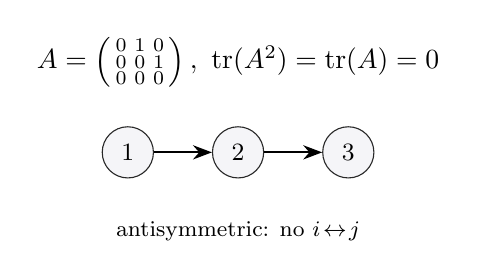
\begin{tikzpicture}
% antisymmetric chain 1->2->3
\begin{scope}
  \node[vtx] (d1) at (0,0) {1};
  \node[vtx] (d2) at (1.4,0) {2};
  \node[vtx] (d3) at (2.8,0) {3};
  \draw[arr] (d1)--(d2); \draw[arr] (d2)--(d3);
  \node at (1.4,-1.0) {\footnotesize antisymmetric: no $i\!\leftrightarrow\!j$};
  \node at (1.4,1.15) {$A=\smallmat{0&1&0\\0&0&1\\0&0&0},\ \tr(A^{2})=\tr(A)=0$};
\end{scope}
\end{tikzpicture}
\end{center}

\noindent\textbf{Why transitivity is the odd one out.} The first four rows are
\emph{linear-algebra} facts: they count things, and counting is what trace does.
Transitivity ($A^{2}\le A$) is a \emph{Boolean} condition --- it asks only
whether a length-$2$ path \emph{exists}, never how many. Existence is not a sum
of a diagonal, so there is no clean trace characterization. This is the honest
boundary of the trace story: \emph{trace lives over linear algebra, transitivity
lives over Boolean algebra.}

\section*{4. The categorical picture: trace $=$ feedback}

Strip away the matrix and only the arrows remain. An \textbf{endorelation}
$R\colon X\to X$ is an arrow from an object to itself; composing it is taking
powers, $R^{k}=R\circ\cdots\circ R$. In a symmetric monoidal category with duals
the trace of an endomorphism $f\colon V\to V$ is the single closed loop
(evaluation~$\varepsilon$ against coevaluation~$\eta$):

\begin{center}
\begin{tikzcd}[column sep=2.1em, row sep=large]
I \arrow[r, "\eta"]
& V\otimes V^{*} \arrow[r, "f\,\otimes\,\id"]
& V\otimes V^{*} \arrow[r, "\text{swap}"]
& V^{*}\otimes V \arrow[r, "\varepsilon"]
& I
\end{tikzcd}
\qquad
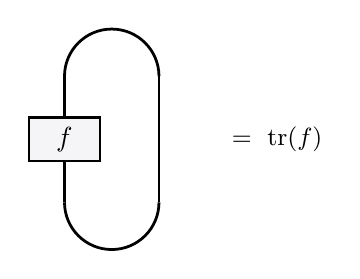
\begin{tikzpicture}[line width=1pt, baseline=0.9cm]
\draw (0.0,0.4) -- (0.0,2.0);
\node[draw, fill=soft, minimum width=0.9cm, minimum height=0.55cm] at (0.0,1.2) {$f$};
\draw (0.0,2.0) arc (180:0:0.6);
\draw (1.2,2.0) -- (1.2,0.4);
\draw (0.0,0.4) arc (-180:0:0.6);
\node at (2.7,1.2) {\small $=\ \tr(f)$};
\end{tikzpicture}
\end{center}

Applied to the adjacency matrix this loop is exactly $\sum_i a_{ii}$; applied to
$A^{k}$ it is $\sum_i(A^{k})_{ii}$. So the three faces of the same idea are:

\begin{center}
\begin{tabular}{@{}l@{\ $=$\ }l@{}}
trace & local invariant: the closed loops / self-feedback of $R$,\\
$R^{k}$ & the relation composed with itself $k$ times,\\
$\tr(R^{k})$ & the \textbf{fixed points of $R^{k}$}: points returning after $k$ steps.\\
\end{tabular}
\end{center}

\noindent This ``count the points that come back'' reading is why traces of
powers pervade graph theory, spectral graph theory, and topology --- the
\textbf{Lefschetz fixed-point theorem} is the same slogan for continuous maps:
an alternating sum of traces on homology counts (with signs) the fixed points of
a self-map. Endorelation, endomorphism, endomap: one loop, many settings.

\section*{5. Where this project lives: the Frobenius endorelation}

Now specialise the object to a finite field $L=\mathbb{F}_{2^{n}}$ of
characteristic $2$, the setting of the \lc{Equation1} formalisation. Two
different ``adjacency'' pictures appear, and the trace loop of \S4 explains both.

\subsection*{5a. Frobenius as a graph --- its cycles are the cosets \bC}

The Frobenius map $\sigma\colon x\mapsto x^{2}$ is a \emph{bijective}
endorelation on $L$ (brick~\bF). A bijection's graph is a permutation matrix
$P$, and its picture is a disjoint union of cycles --- its \textbf{functional
graph}. Here those cycles are precisely the \textbf{cyclotomic cosets}
(brick~\bC): the orbit of an exponent $e$ under doubling mod $2^{n}-1$.

\begin{center}
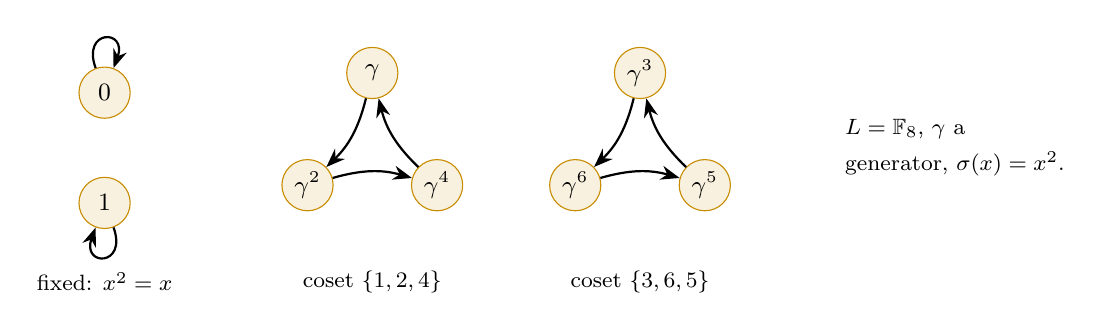
\begin{tikzpicture}
% Frobenius on F_8: two fixed points and two 3-cycles
\begin{scope}
  \node[fld] (z) at (0,0.7) {$0$};
  \draw[arr] (z) to[out=110,in=70,looseness=6] (z);
  \node[fld] (o) at (0,-0.7) {$1$};
  \draw[arr] (o) to[out=-70,in=-110,looseness=6] (o);
  \node at (0,-1.7) {\footnotesize fixed: $x^{2}=x$};
\end{scope}
\begin{scope}[xshift=3.4cm]
  \node[fld] (g1) at (90:0.95)  {$\gamma$};
  \node[fld] (g2) at (210:0.95) {$\gamma^{2}$};
  \node[fld] (g4) at (330:0.95) {$\gamma^{4}$};
  \draw[arr] (g1) to[bend left=16] (g2);
  \draw[arr] (g2) to[bend left=16] (g4);
  \draw[arr] (g4) to[bend left=16] (g1);
  \node at (0,-1.7) {\footnotesize coset $\{1,2,4\}$};
\end{scope}
\begin{scope}[xshift=6.8cm]
  \node[fld] (h1) at (90:0.95)  {$\gamma^{3}$};
  \node[fld] (h2) at (210:0.95) {$\gamma^{6}$};
  \node[fld] (h4) at (330:0.95) {$\gamma^{5}$};
  \draw[arr] (h1) to[bend left=16] (h2);
  \draw[arr] (h2) to[bend left=16] (h4);
  \draw[arr] (h4) to[bend left=16] (h1);
  \node at (0,-1.7) {\footnotesize coset $\{3,6,5\}$};
\end{scope}
\node[align=left] at (10.8,0)
  {\footnotesize $L=\mathbb{F}_{8}$, $\gamma$ a\\[1pt]
   \footnotesize generator, $\sigma(x)=x^{2}$.};
\end{tikzpicture}
\end{center}

\noindent Reading off the trace of powers of this permutation matrix $P$ is now
pure~\S4: $\tr(P^{k})$ counts the elements fixed by $\sigma^{k}$, i.e.\ solutions
of $x^{2^{k}}=x$, i.e.\ the subfield $\mathbb{F}_{2^{\gcd(k,n)}}\cap L$:
\[
\tr(P^{k})=\#\{x\in L: x^{2^{k}}=x\}=2^{\gcd(k,n)} .
\]
For $L=\mathbb{F}_{8}$ ($n=3$): $\tr(P)=\tr(P^{2})=2$ (just $0,1$) and
$\tr(P^{3})=8$ (everything returns) --- the two length-$3$ cosets snap shut
exactly when $3\mid k$. This is the ``cycles of length dividing $k$'' rule of
\S2, now saying \textbf{cyclotomic cosets = Frobenius cycles}, the concrete
content of brick~\bC.

\subsection*{5b. The project's trace is the loop of \S4 --- brick \bL}

The \emph{other} matrix is linear, not Boolean. Fix $x\in L$ and multiply by it:
$m_{x}\colon L\to L,\ y\mapsto x\cdot y$. Viewing $L$ as an $n$-dimensional
$\mathbb{F}_{2}$-vector space, $m_{x}$ has an honest $0/1$-and-beyond matrix over
$\mathbb{F}_{2}$, and the categorical loop of \S4 applied to it is the
\textbf{field trace}. Over $\mathbb{F}_{2}$ that loop unwinds into a Frobenius
sum --- the project's own \lc{Tr}/\lc{truncTrace} (brick~\bL):
\[
\Tr_{L/\mathbb{F}_{2}}(x)\;=\;\tr(m_{x})\;=\;\sum_{i=0}^{n-1}x^{2^{i}} .
\]

\begin{leanbox}
\small
\textbf{Machine-checked in} \lc{Equation1/TraceLibrary.lean}\textbf{:}\\[2pt]
\lc{Tr\_eq\_truncTrace}\ \ ---\ the two trace functions coincide;\\
\lc{Tr\_eq\_algebraMap\_trace}\ \ ---\ $\Tr\,n\,x
=\texttt{algebraMap}\ \mathbb{Z}/2\ L\,\bigl(\texttt{Algebra.trace}\ \mathbb{Z}/2\ L\ x\bigr)$;\\
so the diagonal-sum trace of $m_{x}$ \emph{is} $\sum_{i<n}x^{2^{i}}$
(via \lc{FiniteField.algebraMap\_trace\_eq\_sum\_pow}).
\end{leanbox}

\noindent Notice the pleasing overlap between the two pictures. The summands
$x,x^{2},x^{4},\dots$ of the trace are the images of $x$ under the Frobenius
orbit of \S5a --- \textbf{summing an element around its own coset cycle}. The
feedback loop of \S4 (add up the diagonal of $m_x$) and the fixed-point count of
\S5a (trace of $\sigma^{k}$) are two readings of the one word ``trace'': the
first over linear algebra~\bL, the second over the Boolean/permutation
combinatorics of the cosets~\bC, glued by the Frobenius~\bF.

\section*{6. Does it apply to Dobbertin? --- yes, with one caveat}

\begin{note}
\textbf{Applicable.} The trace $\Tr(x)=\sum_{i<n}x^{2^{i}}$ that Dobbertin uses
to state equation~(1) is exactly the categorical trace of ``multiply by $x$''
(\S5b, verified in \lc{TraceLibrary.lean}), and the doubling/cyclotomic-coset
bookkeeping he uses silently is the Frobenius functional graph of \S5a.\\[3pt]
\textbf{Caveat.} The trace \emph{of powers} identity $\tr(A^{k})=\#$closed walks
is a statement about the $0/1$ adjacency matrix of a general relation; in the
Dobbertin/\lc{Equation1} extract it appears in the specialised
\emph{permutation} form of \S5a ($\tr(\sigma^{k})=2^{\gcd(k,n)}$), not as a
graph-triangle count. The transitivity row of \S3 has, as noted there, no trace
avatar --- and correspondingly no role in this field-trace development.
\end{note}

\vfill
\hrule
\begin{center}\small
Diagrams: TikZ / tikz-cd. Companion to \texttt{TraceMap\_Categorically}
and \texttt{Equation1\_LEGO}. Rebuild with
\texttt{tectonic TracePowers\_Relations.tex}.
\end{center}

\end{document}
